\documentclass[]{llncs} 
\usepackage{amsmath}
\usepackage{verbatim}
\usepackage{datatool}
\usepackage{tikz}
\usetikzlibrary{arrows,shapes}
\usepackage{graphics}


\newcommand{\TODO}[1]{ {\color{red}{#1} }}
\newcommand{\com}[1]{ {\color{blue}{--- #1 ---}}}

\newcommand{\AtMostSeqCard}{AtMostSeqCard }

\author{Valentin Mayer-Eichberger}

\institute{NICTA \\ University of New South Wales \\
\email{valentin.mayer-eichberger@nicta.com.au}}

\title{SAT Encodings for the Car Sequencing Problem}

\begin{document} \maketitle

\section{Introduction}

We will present several encodings of the car sequencing problem and
discuss their differences. First we start with a rather simple and
direct translation of the description of the problem and then gradually
improve this encoding by various techniques. In the construction we will
show how to use partial sums, order encodings and how to compactly
translate cardinality constraints and strengthen propagation by focusing
on the auxiliary variables. 

\section{Motivation}

Our motivation comes from the recent good results of \cite{Siala12} on
the car sequencing benchmark by using a specialized propagator of the
\AtMostSeqCard constraint. This constraint treats a special case of the
Sequence constraint (\cite{Hoeve06}) where the lower bound for the
Amongs is $0$.  Here we will show that there is good  CNF decomposition
that archive compatible results on the instances of benchmarks of in the
CSP$_{\mbox{LIB}}$ \cite{Gent99}. 

\section{Two simple Encoding}

\begin{enumerate}
    \item Encoding by boolean variables $c^k_{i}$ for class $k$ in
        position $i$ and a cardinality constraint on the total number of
        classes on the sequence and cardinality constraints on each sub
        window restricting the capacity on options. No further global
        constraints and cardinality constraints translated by standard
        SAT encoding. (referred to as $E_1$)
    \item As 1) but introducing auxiliary variables $o^l_{i}$ for option
        $l$ in position $i$ to encode the capacity constraints on options.
        (referred to as $E_2$). 
\end{enumerate}


\section{Encoding of a single \AtMostSeqCard Constraint}


We will first show how to encode a cardinality constraint with a counter
encoding (\TODO{First publication?}) and then integrate the AtMostSeq
by reusing the auxiliary variables of the counter encoding. 

Over this whole section we will work with the following notation. Given
a set of consecutive positions $P=\{1\ldots n\}$ and a property that
holds at a position $i\in P$ iff the boolean variable $x_i$ is true. 

\subsection{Encoding of Counters}

We show how to encode a cardinality constraint of the following form 

$$ \sum_{i\in \{1\ldots n\}} x_{i} = d $$

where $x_i$ are boolean variables and $d$ is a fixed value. The encoding
given here is named a counter encoding. The idea is to introduce
auxiliary variables to denote cumulative sums with order encoding
(\cite{Tamura09}) on these variables. 

We introduce the following boolean variables (representing cumulative sums): 

\begin{itemize}
    \item $y_{i,j}$ is true iff in the positions $1 \ldots i$ the
        property holds at least $j$ times.        
\end{itemize}

The following formula clarifies the relationship between $x$ and $y$.

$$ y_{i,j} \iff (j \leq \sum_{l=0}^{i} x_{l}) $$


\begin{figure}
\centering 
\caption{The variables $y_{i,j}$ with $d=2$ over a sequence of 10
variables. By preprocessing the variables corresponding to the cells
containing $U$($L$) and above(below) are set to false (true).  The
question mark identifies yet unassigned variables.}
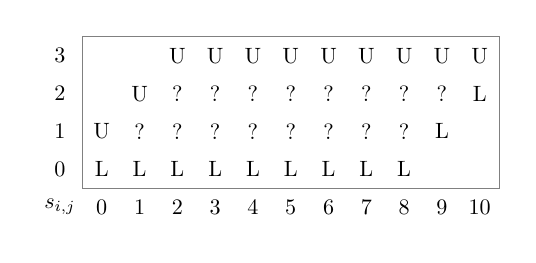
\begin{tikzpicture}[scale=0.8,every node/.style={scale=0.8}]
\node [matrix,ampersand replacement=\&,nodes={minimum size=6mm}]
%,nodes={fill=blue!20,minimum size=5mm}] 
    {
        \node {3}; \& \node (x) { }; \& \node { }; \& \node {U}; \& \node {U}; \& \node {U}; \& \node {U}; \& \node {U}; \& \node {U}; \& \node {U}; \& \node {U}; \& \node {U}; \\
        \node {2}; \& \node { }; \& \node {U}; \& \node {?}; \& \node {?}; \& \node {?}; \& \node {?}; \& \node {?}; \& \node {?}; \& \node {?}; \& \node {?}; \& \node {L}; \\
        \node {1}; \& \node {U}; \& \node {?}; \& \node {?}; \& \node {?}; \& \node {?}; \& \node {?}; \& \node {?}; \& \node {?}; \& \node {?}; \& \node {L}; \& \node { }; \\
        \node {0}; \& \node {L}; \& \node {L}; \& \node {L}; \& \node {L}; \& \node {L}; \& \node {L}; \& \node {L}; \& \node {L}; \& \node {L}; \& \node { }; \& \node (y) { }; \\
        \node {$s_{i,j}$}; \& \node {0}; \& \node {1}; \& \node {2}; \& \node {3}; \& \node {4}; \& \node {5}; \& \node {6}; \& \node {7}; \& \node {8}; \& \node {9}; \& \node {10}; \\
};
\draw[gray] (x.north west) rectangle (y.south east);
\end{tikzpicture}


\label{ex:1}
\end{figure}

The following binary clauses relate the variables $y$ among each other:

\begin{equation} \label{eq:1}
    \bigwedge_{i \in \{0\ldots n-1\}} \bigwedge_{j \in\{0..d+1\}}
    \neg y_{i,j} \vee y_{i+1,j}
\end{equation}

\begin{equation} \label{eq:2}
    \bigwedge_{i \in \{1..n\}} \bigwedge_{j\in \{1..d+1\}}
    \neg y_{i,j} \vee y_{i-1,j-1}
\end{equation}

These clauses restrict assignments of the auxiliary variables to 
represent a counter.

Now we need to relate these variables to $x$.  First we restrict the
counter not to increase if $x_{i}$ is false:

\begin{equation} \label{eq:3}
    \bigwedge_{i \in \{1\ldots n\}} \bigwedge_{j\in\{0..d+1\}}
    x_{i} \vee \neg y_{i,j} \vee y_{i-1,j}
\end{equation}

Second we define clauses that push  the counter up if $x_i$ is true. 

\begin{equation} \label{eq:4}
    \bigwedge_{i \in \{0\ldots n-1\}} \bigwedge_{j\in\{0..d\}}
    \neg x_{i+1} \vee \neg y_{i,j} \vee y_{i+1,j+1}
\end{equation}

Now we finally have to "initialize" the counter. 

\begin{equation} \label{eq:5}
    y_{n,d} \wedge \left (\bigwedge_{i\in\{0\ldots n\}} y_{i,0} \right )\wedge \neg
    y_{0,1} \wedge \left(\bigwedge_{i\in\{0\ldots n\}} \neg
        y_{i,d+1}\right )
\end{equation}

It should be mentioned that formula (\ref{eq:5}) defines the counter to
accept exactly $d$ occurrences. However not needed for later, we can
easily change the initialiser to define a constraint of at most $d$ or
at least $d$. 

\begin{proposition} 
    Clauses (\ref{eq:1}) to (\ref{eq:4}) encode the cardinality
    constraint $ \sum_{i} x_{i} = d $ and UP enforce GAC on any partial
    assignment on variables $x_i$. 
\end{proposition}

\begin{proof}
    We sketch the proof: Clauses (\ref{eq:3}) and (\ref{eq:4}) translate
    directly from the definition of the auxiliary variables representing
    cumulative sums.  Clauses (\ref{eq:1}) and (\ref{eq:2}) represent
    the domain encoding of the bounds on the cumulative sums. 
    
    For GAC we need to show that given a partial assignment and assuming
    a variable $x_i$ is not unit although should have been propagated.
    This will lead to a contradiction by case analysis on true and false
    of $x_i$ and the clauses (\ref{eq:3}) and (\ref{eq:4}). In either
    case we are left with at least one binary clauses with index $j$ as
    UP did not enforce $x_i$ and by the definition of $y_{i,j}$ we have a
    contradiction. 
\end{proof}

Note that the given encoding is not the most compact for a single
cardinality constraint.  However, the auxiliary variables are reused in
the following section to encode a sequence of AtMost constraints.        


\begin{figure}
\centering 
\caption{Taking the counter of Figure \ref{ex:1} and let $x_{i}$ be
true for position 2 and 7. Then the resulting assignment after UP to the
auxiliary variables is given in this table. } 
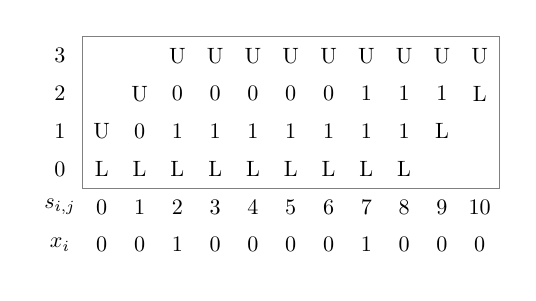
\begin{tikzpicture}[scale=0.8,every node/.style={scale=0.8}]    
\node [matrix,ampersand replacement=\&,nodes={minimum size=6mm}]
%,nodes={fill=blue!20,minimum size=5mm}] 
    {
        \node {3}; \& \node (x) { }; \& \node { }; \& \node {U}; \& \node {U}; \& \node {U}; \& \node {U}; \& \node {U}; \& \node {U}; \& \node {U}; \& \node {U}; \& \node {U}; \\
        \node {2}; \& \node { }; \& \node {U}; \& \node {0}; \& \node {0}; \& \node {0}; \& \node {0}; \& \node {0}; \& \node {1}; \& \node {1}; \& \node {1}; \& \node {L}; \\
        \node {1}; \& \node {U}; \& \node {0}; \& \node {1}; \& \node {1}; \& \node {1}; \& \node {1}; \& \node {1}; \& \node {1}; \& \node {1}; \& \node {L}; \& \node { }; \\
        \node {0}; \& \node {L}; \& \node {L}; \& \node {L}; \& \node {L}; \& \node {L}; \& \node {L}; \& \node {L}; \& \node {L}; \& \node {L}; \& \node { }; \& \node (y) { }; \\
        \node {$s_{i,j}$}; \& \node {0}; \& \node {1}; \& \node {2}; \& \node {3}; \& \node {4}; \& \node {5}; \& \node {6}; \& \node {7}; \& \node {8}; \& \node {9}; \& \node {10}; \\
        \node {$x_{i}$}; \& \node {0}; \& \node {0}; \& \node {1}; \& \node {0}; \& \node {0}; \& \node {0}; \& \node {0}; \& \node {1}; \& \node {0}; \& \node {0}; \& \node {0}; \\
};
\draw[gray] (x.north west) rectangle (y.south east);
\end{tikzpicture}


\label{ex:2}
\end{figure}


\subsection{Extending to \AtMostSeqCard}

\AtMostSeqCard is a specialized Sequence constraint: Given a sequence of
boolean variables of which exactly $d$ have to be true and each window
of size $q$ cannot contain more than $u$ true variables. More formally: 

$$ \text{\AtMostSeqCard}(u,q,d,[x_{1},\ldots,x_{n}]) \iff (\sum_{i=1}^n
x_{i} = d) \wedge \bigwedge_{i=1}^{n-q}(\sum_{l=1}^q x_{i+l} \leq u )$$

To detect dis-entailment on this constraint by the CNF decomposition we
propose to decompose the cardinality constraints by the counter encoding
of the previous section and add the following binary clauses:

\begin{equation} \label{eq:6}
    \bigwedge_{\substack{i \in \{1 \ldots n\} \\ i-q \geq 0}}
    \bigwedge_{\substack{j\in\{1\ldots d+1\}\\ j-u \geq 0}}
    \neg y_{i,j} \vee y_{i-q,j-u}
\end{equation}               


\begin{theorem}
    The clauses of counter encoding (\ref{eq:1}) to (\ref{eq:5}) with
    the clauses of (\ref{eq:6}) are logically equivalent to the
    \AtMostSeqCard. Moreover it detects dis-entailment with UP and thus
    GAC with failed literal test. 
\end{theorem}


\begin{proof}
    Idea: We need to show that together with GAC on the cardinality
    constraints and clauses (\ref{eq:6}) we enforce bounds consistency
    on the auxiliary cumulative sums. The proof could use the
    construction in \cite{Bacchus07} on the sequence constraint to show
    dis-entailment and the idea \cite{Brand07} to enforce bounds
    consistency on the cumulative sums. 
\end{proof}


\subsection{Size of Encoding} 

Let $s = (n\cdot d-\text{upper and lower triangle})$, then we require $s$
auxiliary variables and $3\cdot (s+n)$ binary clauses and $2\cdot (s+n)$ ternary
clauses. The term $n\cdot d$ dominates and the precise number of
variables can be computed by the hight $d$ and the slope $u/q$ and some
basic algebra, which leads to $d\cdot(u-q+\frac{d \cdot q}{u}) $. So the
number of variables $s$ are

$$ s = d \cdot n - d \cdot(u-q+\frac{d \cdot q}{u}) $$

Thus the size of this encoding lies in $O(nd)$, but can be more compact
if $q$ and $u$ are rather strict and/or $d$ is close to $n$. For example
\AtMostSeqCard$(u=4,q=8,d=12,n=22)$ would have 

$ 12\cdot 22- 12\cdot ( 4-8+\frac{12 \cdot 8}{4}) = 24$ variables. 

%\begin{figure}
%\centering 
%\caption{A graphical representation of the 6 rules for counters and the
%\AtMostSeqCard constraint. }
%%\begin{tikzpicture}
\draw (-2,0) node {(1)};
\node [bend angle=45,matrix,ampersand replacement=\&,nodes={shape=rectangle,minimum size=6mm}]
{
    \node {}; \& \node[draw] (x) { }; \\
    \node[draw] (y) {}; \& \node { }; \\
};
\draw[bend angle=45,->, sloped, above] (x.west) -- (y.north); 
%    {
%        \node {3}; \& \node (x) { }; \& \node { }; \& \node {U}; \& \node {U}; \& \node {U}; \& \node {U}; \& \node {U}; \& \node {U}; \& \node {U}; \& \node {U}; \& \node {U}; \\
%        \node {2}; \& \node { }; \& \node {U}; \& \node {?}; \& \node {?}; \& \node {?}; \& \node {?}; \& \node {?}; \& \node {?}; \& \node {?}; \& \node {?}; \& \node {L}; \\
%        \node {1}; \& \node {U}; \& \node {?}; \& \node {?}; \& \node {?}; \& \node {?}; \& \node {?}; \& \node {?}; \& \node {?}; \& \node {?}; \& \node {L}; \& \node { }; \\
%        \node {0}; \& \node {L}; \& \node {L}; \& \node {L}; \& \node {L}; \& \node {L}; \& \node {L}; \& \node {L}; \& \node {L}; \& \node {L}; \& \node { }; \& \node (y) { }; \\
%        \node {j/i}; \& \node {0}; \& \node {1}; \& \node {2}; \& \node {3}; \& \node {4}; \& \node {5}; \& \node {6}; \& \node {7}; \& \node {8}; \& \node {9}; \& \node {10}; \\
%};
%\draw[gray] (x.north west) rectangle (y.south east);
\end{tikzpicture}


%\end{figure}

\TODO{Give two references here}: \cite{Bacchus07} and \cite{Bessiere09}
on decompositions of the sequence constraint and failed literal test and
discuss size of the encoding. 

The power of the binary clauses are best illustrated by reusing the
example \cite{Siala12} in Figures \ref{fig3} and \ref{fig4}.

\begin{figure}
\centering 
\caption{Here we analyse the initial state of variables for a constraint
with $u=4,q=8,d=12,n=22$. In this example we see that $x_{7}$, $x_{8}$,
$x_{15}$ and $x_{16}$ should be false, this is detected by UP.}
\begin{tikzpicture}
\node [matrix,ampersand replacement=\&,nodes={minimum size=6mm}]
%,nodes={fill=blue!20,minimum size=5mm}] 
    {
\node{13}; \& \node (x) { }; \& \node { }; \& \node { }; \& \node { }; \& \node { }; \& \node { }; \& \node { }; \& \node { }; \& \node { }; \& \node { }; \& \node { }; \& \node { }; \& \node { }; \& \node { }; \& \node { }; \& \node { }; \& \node { }; \& \node { }; \& \node { }; \& \node { }; \& \node {U}; \& \node {U}; \& \node {U}; \\
\node{12}; \& \node { }; \& \node { }; \& \node { }; \& \node { }; \& \node { }; \& \node { }; \& \node { }; \& \node { }; \& \node { }; \& \node { }; \& \node { }; \& \node { }; \& \node { }; \& \node { }; \& \node { }; \& \node { }; \& \node { }; \& \node { }; \& \node { }; \& \node {U}; \& \node {?}; \& \node {?}; \& \node {L}; \\
\node{11}; \& \node { }; \& \node { }; \& \node { }; \& \node { }; \& \node { }; \& \node { }; \& \node { }; \& \node { }; \& \node { }; \& \node { }; \& \node { }; \& \node { }; \& \node { }; \& \node { }; \& \node { }; \& \node { }; \& \node { }; \& \node { }; \& \node {U}; \& \node {?}; \& \node {?}; \& \node {L}; \& \node { }; \\
\node{10}; \& \node { }; \& \node { }; \& \node { }; \& \node { }; \& \node { }; \& \node { }; \& \node { }; \& \node { }; \& \node { }; \& \node { }; \& \node { }; \& \node { }; \& \node { }; \& \node { }; \& \node { }; \& \node { }; \& \node { }; \& \node {U}; \& \node {?}; \& \node {?}; \& \node {L}; \& \node { }; \& \node { }; \\
\node{9}; \& \node { }; \& \node { }; \& \node { }; \& \node { }; \& \node { }; \& \node { }; \& \node { }; \& \node { }; \& \node { }; \& \node { }; \& \node { }; \& \node { }; \& \node {U}; \& \node {U}; \& \node {U}; \& \node {U}; \& \node {U}; \& \node {?}; \& \node {?}; \& \node {L}; \& \node { }; \& \node { }; \& \node { }; \\
\node{8}; \& \node { }; \& \node { }; \& \node { }; \& \node { }; \& \node { }; \& \node { }; \& \node { }; \& \node { }; \& \node { }; \& \node { }; \& \node { }; \& \node {U}; \& \node {?}; \& \node {?}; \& \node {L}; \& \node {L}; \& \node {L}; \& \node {L}; \& \node {L}; \& \node { }; \& \node { }; \& \node { }; \& \node { }; \\
\node{7}; \& \node { }; \& \node { }; \& \node { }; \& \node { }; \& \node { }; \& \node { }; \& \node { }; \& \node { }; \& \node { }; \& \node { }; \& \node {U}; \& \node {?}; \& \node {?}; \& \node {L}; \& \node { }; \& \node { }; \& \node { }; \& \node { }; \& \node { }; \& \node { }; \& \node { }; \& \node { }; \& \node { }; \\
\node{6}; \& \node { }; \& \node { }; \& \node { }; \& \node { }; \& \node { }; \& \node { }; \& \node { }; \& \node { }; \& \node { }; \& \node {U}; \& \node {?}; \& \node {?}; \& \node {L}; \& \node { }; \& \node { }; \& \node { }; \& \node { }; \& \node { }; \& \node { }; \& \node { }; \& \node { }; \& \node { }; \& \node { }; \\
\node{5}; \& \node { }; \& \node { }; \& \node { }; \& \node { }; \& \node {U}; \& \node {U}; \& \node {U}; \& \node {U}; \& \node {U}; \& \node {?}; \& \node {?}; \& \node {L}; \& \node { }; \& \node { }; \& \node { }; \& \node { }; \& \node { }; \& \node { }; \& \node { }; \& \node { }; \& \node { }; \& \node { }; \& \node { }; \\
\node{4}; \& \node { }; \& \node { }; \& \node { }; \& \node {U}; \& \node {?}; \& \node {?}; \& \node {L}; \& \node {L}; \& \node {L}; \& \node {L}; \& \node {L}; \& \node { }; \& \node { }; \& \node { }; \& \node { }; \& \node { }; \& \node { }; \& \node { }; \& \node { }; \& \node { }; \& \node { }; \& \node { }; \& \node { }; \\
\node{3}; \& \node { }; \& \node { }; \& \node {U}; \& \node {?}; \& \node {?}; \& \node {L}; \& \node { }; \& \node { }; \& \node { }; \& \node { }; \& \node { }; \& \node { }; \& \node { }; \& \node { }; \& \node { }; \& \node { }; \& \node { }; \& \node { }; \& \node { }; \& \node { }; \& \node { }; \& \node { }; \& \node { }; \\
\node{2}; \& \node { }; \& \node {U}; \& \node {?}; \& \node {?}; \& \node {L}; \& \node { }; \& \node { }; \& \node { }; \& \node { }; \& \node { }; \& \node { }; \& \node { }; \& \node { }; \& \node { }; \& \node { }; \& \node { }; \& \node { }; \& \node { }; \& \node { }; \& \node { }; \& \node { }; \& \node { }; \& \node { }; \\
\node{1}; \& \node {U}; \& \node {?}; \& \node {?}; \& \node {L}; \& \node { }; \& \node { }; \& \node { }; \& \node { }; \& \node { }; \& \node { }; \& \node { }; \& \node { }; \& \node { }; \& \node { }; \& \node { }; \& \node { }; \& \node { }; \& \node { }; \& \node { }; \& \node { }; \& \node { }; \& \node { }; \& \node { }; \\
\node{0}; \& \node {L}; \& \node {L}; \& \node {L}; \& \node { }; \& \node { }; \& \node { }; \& \node { }; \& \node { }; \& \node { }; \& \node { }; \& \node { }; \& \node { }; \& \node { }; \& \node { }; \& \node { }; \& \node { }; \& \node { }; \& \node { }; \& \node { }; \& \node { }; \& \node { }; \& \node { }; \& \node (y) { }; \\
\node{j/i}; \& \node {0}; \& \node {1}; \& \node {2}; \& \node {3}; \& \node {4}; \& \node {5}; \& \node {6}; \& \node {7}; \& \node {8}; \& \node {9}; \& \node {10}; \& \node {11}; \& \node {12}; \& \node {13}; \& \node {14}; \& \node {15}; \& \node {16}; \& \node {17}; \& \node {18}; \& \node {19}; \& \node {20}; \& \node {21}; \& \node {22}; \\
\node{$x_i$}; \& \node { }; \& \node { }; \& \node { }; \& \node { }; \&
        \node { }; \& \node { }; \& \node { }; \& \node {\textbf{0}}; \&
        \node {\textbf{0}}; \& \node { }; \& \node { }; \& \node { }; \&
        \node { }; \& \node { }; \& \node { }; \& \node {\textbf{0}}; \&
        \node {\textbf{0}}; \& \node { }; \& \node { }; \& \node { }; \& \node { }; \& \node { }; \& \node { }; \\
};
\draw[gray] (x.north west) rectangle (y.south east);
\end{tikzpicture}


\label{fig3}
\end{figure}

\begin{figure}
\centering 
\caption{State of the auxiliary variables for $u=4,q=8,d=12,n=22$ and
    choices $x_{1}$ and $x_{13}$ to true and $x_{12}$, $x_{14}$ and
    $x_{21}$ to false. Notice the amount of propagation due to the
    clauses of the \AtMostSeqCard constraint, also notice that variable
$x_{1}$ was a redundant choice. Normal font= choice, bold = propagated,
()= propagated before, green arrow positive implication, red arrow
negative implication by (\ref{eq:6}).}
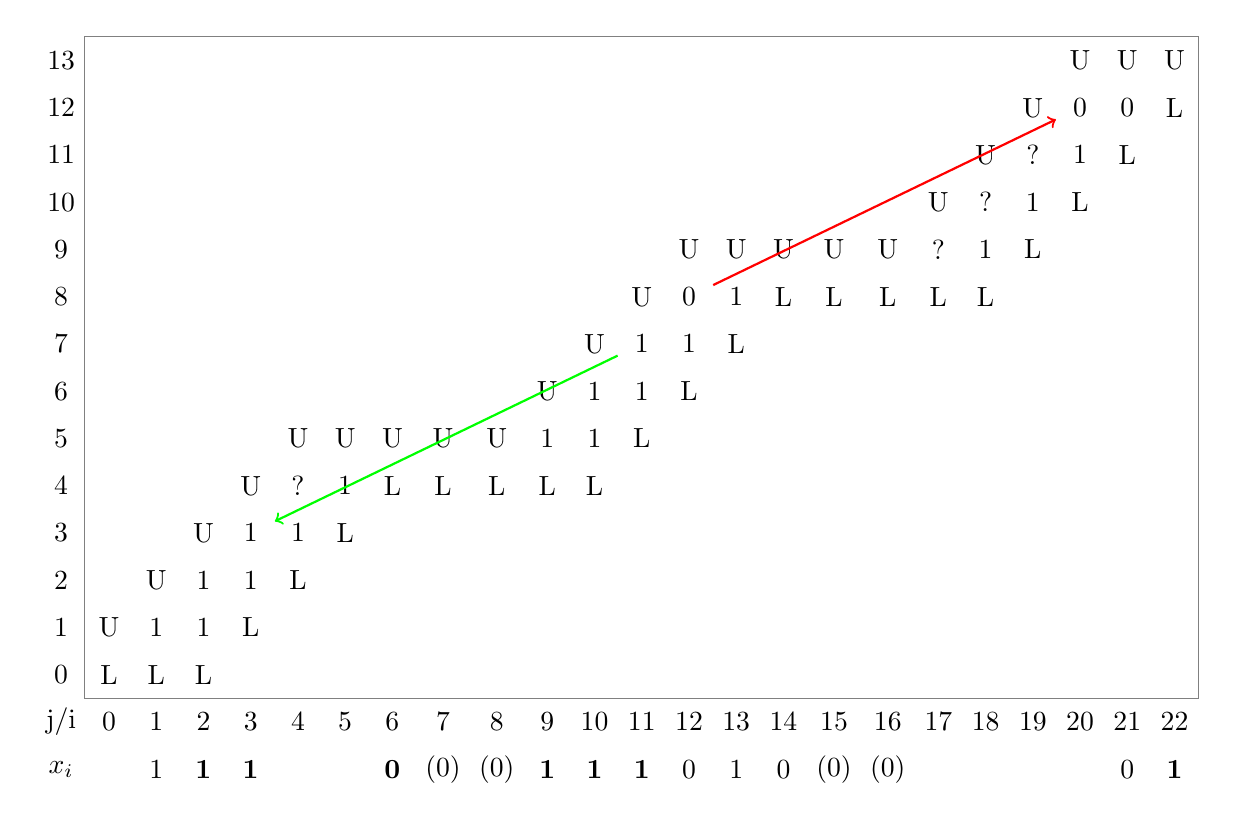
\begin{tikzpicture}
\node [matrix,ampersand replacement=\&,nodes={minimum size=6mm}]
    {
\node {13}; \& \node (x) { }; \& \node { }; \& \node { }; \& \node { }; \& \node { }; \& \node { }; \& \node { }; \& \node { }; \& \node { }; \& \node { }; \& \node { }; \& \node { }; \& \node { }; \& \node { }; \& \node { }; \& \node { }; \& \node { }; \& \node { }; \& \node { }; \& \node { }; \& \node {U}; \& \node {U}; \& \node {U}; \\
\node {12}; \& \node { }; \& \node { }; \& \node { }; \& \node { }; \&
        \node { }; \& \node { }; \& \node { }; \& \node { }; \& \node {
    }; \& \node { }; \& \node { }; \& \node { }; \& \node { }; \& \node
        { }; \& \node { }; \& \node { }; \& \node { }; \& \node { }; \&
        \node { }; \& \node {U}; \& \node (b) {0}; \& \node {0}; \& \node {L}; \\
\node {11}; \& \node { }; \& \node { }; \& \node { }; \& \node { }; \& \node { }; \& \node { }; \& \node { }; \& \node { }; \& \node { }; \& \node { }; \& \node { }; \& \node { }; \& \node { }; \& \node { }; \& \node { }; \& \node { }; \& \node { }; \& \node { }; \& \node {U}; \& \node {?}; \& \node {1}; \& \node {L}; \& \node { }; \\
\node {10}; \& \node { }; \& \node { }; \& \node { }; \& \node { }; \& \node { }; \& \node { }; \& \node { }; \& \node { }; \& \node { }; \& \node { }; \& \node { }; \& \node { }; \& \node { }; \& \node { }; \& \node { }; \& \node { }; \& \node { }; \& \node {U}; \& \node {?}; \& \node {1}; \& \node {L}; \& \node { }; \& \node { }; \\
\node {9}; \& \node { }; \& \node { }; \& \node { }; \& \node { }; \& \node { }; \& \node { }; \& \node { }; \& \node { }; \& \node { }; \& \node { }; \& \node { }; \& \node { }; \& \node {U}; \& \node {U}; \& \node {U}; \& \node {U}; \& \node {U}; \& \node {?}; \& \node {1}; \& \node {L}; \& \node { }; \& \node { }; \& \node { }; \\
\node {8}; \& \node { }; \& \node { }; \& \node { }; \& \node { }; \& \node { }; \& \node { }; \& \node { }; \& \node { }; \& \node { }; \& \node { }; \& \node { }; \& \node {U}; \& \node (a) {0}; \& \node {1}; \& \node {L}; \& \node {L}; \& \node {L}; \& \node {L}; \& \node {L}; \& \node { }; \& \node { }; \& \node { }; \& \node { }; \\
\node {7}; \& \node { }; \& \node { }; \& \node { }; \& \node { }; \&
        \node { }; \& \node { }; \& \node { }; \& \node { }; \& \node {
    }; \& \node { }; \& \node {U}; \& \node (c) {1}; \& \node {1}; \& \node {L}; \& \node { }; \& \node { }; \& \node { }; \& \node { }; \& \node { }; \& \node { }; \& \node { }; \& \node { }; \& \node { }; \\
\node {6}; \& \node { }; \& \node { }; \& \node { }; \& \node { }; \& \node { }; \& \node { }; \& \node { }; \& \node { }; \& \node { }; \& \node {U}; \& \node {1}; \& \node {1}; \& \node {L}; \& \node { }; \& \node { }; \& \node { }; \& \node { }; \& \node { }; \& \node { }; \& \node { }; \& \node { }; \& \node { }; \& \node { }; \\
\node {5}; \& \node { }; \& \node { }; \& \node { }; \& \node { }; \& \node {U}; \& \node {U}; \& \node {U}; \& \node {U}; \& \node {U}; \& \node {1}; \& \node {1}; \& \node {L}; \& \node { }; \& \node { }; \& \node { }; \& \node { }; \& \node { }; \& \node { }; \& \node { }; \& \node { }; \& \node { }; \& \node { }; \& \node { }; \\
\node {4}; \& \node { }; \& \node { }; \& \node { }; \& \node {U}; \& \node {?}; \& \node {1}; \& \node {L}; \& \node {L}; \& \node {L}; \& \node {L}; \& \node {L}; \& \node { }; \& \node { }; \& \node { }; \& \node { }; \& \node { }; \& \node { }; \& \node { }; \& \node { }; \& \node { }; \& \node { }; \& \node { }; \& \node { }; \\
        \node {3}; \& \node { }; \& \node { }; \& \node {U}; \& \node
        (d) {1}; \& \node {1}; \& \node {L}; \& \node { }; \& \node { }; \& \node { }; \& \node { }; \& \node { }; \& \node { }; \& \node { }; \& \node { }; \& \node { }; \& \node { }; \& \node { }; \& \node { }; \& \node { }; \& \node { }; \& \node { }; \& \node { }; \& \node { }; \\
\node {2}; \& \node { }; \& \node {U}; \& \node {1}; \& \node {1}; \& \node {L}; \& \node { }; \& \node { }; \& \node { }; \& \node { }; \& \node { }; \& \node { }; \& \node { }; \& \node { }; \& \node { }; \& \node { }; \& \node { }; \& \node { }; \& \node { }; \& \node { }; \& \node { }; \& \node { }; \& \node { }; \& \node { }; \\
\node {1}; \& \node {U}; \& \node {1}; \& \node {1}; \& \node {L}; \& \node { }; \& \node { }; \& \node { }; \& \node { }; \& \node { }; \& \node { }; \& \node { }; \& \node { }; \& \node { }; \& \node { }; \& \node { }; \& \node { }; \& \node { }; \& \node { }; \& \node { }; \& \node { }; \& \node { }; \& \node { }; \& \node { }; \\
\node {0}; \& \node {L}; \& \node {L}; \& \node {L}; \& \node { }; \& \node { }; \& \node { }; \& \node { }; \& \node { }; \& \node { }; \& \node { }; \& \node { }; \& \node { }; \& \node { }; \& \node { }; \& \node { }; \& \node { }; \& \node { }; \& \node { }; \& \node { }; \& \node { }; \& \node { }; \& \node { }; \& \node (y) { }; \\
\node {j/i}; \& \node {0}; \& \node {1}; \& \node {2}; \& \node {3}; \& \node {4}; \& \node {5}; \& \node {6}; \& \node {7}; \& \node {8}; \& \node {9}; \& \node {10}; \& \node {11}; \& \node {12}; \& \node {13}; \& \node {14}; \& \node {15}; \& \node {16}; \& \node {17}; \& \node {18}; \& \node {19}; \& \node {20}; \& \node {21}; \& \node {22}; \\
        \node{$x_i$}; \& \node {}; \& \node {1}; \& \node {\textbf{1}}; \& \node { \textbf{1}}; \& \node { }; \& \node { }; \& \node {\textbf{0} }; \& \node {(0)}; \& \node {(0)}; \& \node {\textbf{1} }; \& \node {\textbf{1} }; \& \node {\textbf{1} }; \& \node {0}; \& \node {1}; \& \node {0}; \& \node {(0)}; \& \node {(0)}; \& \node { }; \& \node { }; \& \node { }; \& \node { }; \& \node {0}; \& \node {\textbf{1}}; \\
};
\draw[thick,red,->, sloped, above] (a) -- (b); 
\draw[thick,green,->,bend right] (c) -- (d); 
\draw[gray] (x.north west) rectangle (y.south east);
\end{tikzpicture}       

\label{fig4}
\end{figure}                                                

\begin{figure}
\centering 
\caption{ Example where the the failed literal test detects
dis-entailment.  Let $u=1$,$q=2$,$d=2$,$n=5$ and let $x_3=1$, then UP
does not enforce $x_2=0$ nor $x_4=0$. Setting them to true will lead to
a conflict by UP through clauses (\ref{eq:1}),(\ref{eq:2}) and
(\ref{eq:6}).}
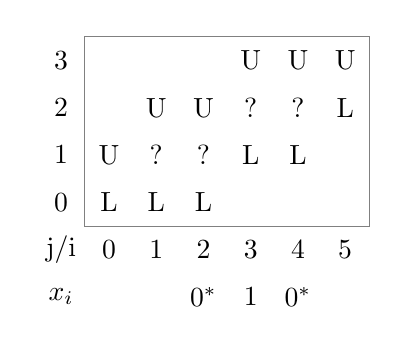
\begin{tikzpicture}
\node [matrix,ampersand replacement=\&,nodes={minimum size=6mm}]
%,nodes={fill=blue!20,minimum size=5mm}] 
    {
        \node {3}; \& \node (x) { }; \& \node { }; \& \node {}; \& \node {U}; \& \node {U}; \& \node {U}; \\
        \node {2}; \& \node { }; \& \node {U}; \& \node {U}; \& \node {?}; \& \node {?}; \& \node {L}; \\
        \node {1}; \& \node {U}; \& \node {?}; \& \node {?}; \& \node {L}; \& \node {L}; \& \node {}; \\
        \node {0}; \& \node {L}; \& \node {L}; \& \node {L}; \& \node {}; \& \node {}; \& \node (y) {};  \\
        \node {j/i}; \& \node {0}; \& \node {1}; \& \node {2}; \& \node {3}; \& \node {4}; \& \node {5}; \\
        \node {$x_{i}$}; \& \node {}; \& \node {}; \& \node {$0^*$}; \& \node {1}; \& \node {$0^*$}; \& \node {}; \\
};
\draw[gray] (x.north west) rectangle (y.south east);
\end{tikzpicture}



\label{ex:5}
\end{figure}


\section{Encoding of Carsequencing}


Let $C$ be the index set identifying a class and $O$ be the index set
for options. The instance for a car sequencing problem is given by a
mapping $m : C\rightarrow 2^O$, relating to each class a set of options.
For each class we have a cardinality constraint and for each option a
AtMostSeq constraint. From this we can construct for each option and for
each class a \AtMostSeqCard constraint on the sequence of the plan
(since all classes have to be assigned we know the exact number of
options).  Each such \AtMostSeqCard constraint is decomposed to CNF. 


The second part of the encoding relates the counter for cars and for
options as in the problem specification.  We will present two ways to do
so. 

\begin{itemize}
    \item Relating variables for cars and options
    \item Relating auxiliary variables in the counter encoding of cars
        and options. 
\end{itemize}

For clarity we introduce two types of variables. Variables $c$ denoting
variables regarding cars and variables $o$ denoting variables regarding
options. Super and subscripts identify the precise meaning of the
variable. For the variables that identify weather a car $k\in C$ or a
option $l\in O$ is at position $i$ we introduce $c^k_i$ and $o^l_j$,
notice that these variables correspond to the single variable of $x_i$
of the construction in the previous section. The for the counter
variables $y$ we denote by $\hat{c}^k_{i,j}$ and $\hat{o}^l_{i,j}$. 


\subsection{Relating Cars and Option directly}

In the first encoding we relate classes and options on each position.
This is done by the following clauses.  Let $m':O \rightarrow 2^C$ be
the reverse mapping relating an option to its set of classes. Then

\begin{equation}
    \bigwedge_{i\in \{1\ldots n\}} \bigwedge_{\substack{k \in C \\ l \in
    m(k)}} \neg c^k_{i} \vee o^l_{i}
\end{equation}

and the support

\begin{equation}
    \bigwedge_{i \in \{1\dots n\}} \bigwedge_{l\in O} \left(\neg o^l_{i} \vee
    \bigvee_{k \in m'(l)} c^k_{i}\right)
\end{equation}

need to hold. We refer to this encoding as $E_3$. 

Remark: Notice in an ASP encoding this would be modelled by one rule and
the completion semantics covers for the reverse case. 

\subsection{An Encoding only Relating Auxiliary Variables}

Here we will show that omit variables $c^k_{i}$ and $o^l_{i}$. The
encoding builds entirely on the auxiliary variables $\hat{c}^k_{i,j}$
and $\hat{o}^l_{i,j}$ and their relationship.

This encoding will enforce more global propagation that is not covered
by the previous encodings and as such has stronger properties taking the
auxiliary variables into account! \TODO{give example which propagation
is missing}.

Here the idea: 

For each position in the sequence, the sum of true $\hat{c}^k$ for cars
$k$ that have option $l$ need to be the same size as the number of true
$\hat{o}^l$ for option $l$. As a formula, for all positions $i$ and
options $ l \in O$ it has to hold: 

$$ \sum_{j} o^l_{i,j} = \sum_{k \in m'(l)} \sum_j c^k_{i,j} $$

With this we only miss the restriction that exactly one class per
position. This can be enforced by introducing an option that all classes
have. 

The decomposition of the above equality  can be done by a sorting
network (as in \cite{Een06}, sorting networks see \cite{Batcher68}) and
the size should be $n\cdot log^2 (d) $ in the hight $d$ of the counter.
For pure cardinality constraints this can be improved in a CNF encoding
as in \cite{Asin11,Codish10}, but here we face an equivalence which
needs a full sorter. Maybe the recursive structure of the cumulative sum
can be exploited in this construction, since in position $i-1$ we sorted
the sequence with up to one difference with positions left and right of
it. 

We refer to this encoding as $E_4$.

\section{CP Model: Cumulative Sums}

This encoding uses the idea behind sequence constraint in \cite{Brand07}
and we adapt it here for the \AtMostSeqCard with redundant constraints.
Let $S_i$ be an integer variable encoding the partial sum of positions
$1\ldots n$. Then we post the following linear constraints and enforce
bounds consistency on all. For all positions $i$ and demands $d$, and
the mapping between cars $k$ and options $l$: 

\begin{align}
    S_{i-1} & \leq S_i \\
    S_i & \leq S_{i-1} + 1 \\
    S_i & = S_{i-1} + x_i \\
    S_i & \leq S_{i-q} + u  \\
    S_n & = d \\
    S^l_i & = \sum_{k \in m'(l)} S^k_i \\
    i & = \sum_{k \in C} S^k_i
\end{align}

With this set of constraints we can simulate the SAT encodings $E_3$ and $E_4$, depending on
the choice of constraints and variables. 

\subsection{Symmetry Breaking Constraints}

A simple symmetry breaking constraint is restricting the class of the first car in the sequence to be of a lower or
equal class than the last car in sequence. This is correct we can read the sequence from the beginning to the end or the
other way around and the capacity constraints are equally satisfied. There is one interesting point to be made,
formulating this constraint with boolean variables. We can either multiply all combinations of violated combinations of
cars. The size is  $n^2$ binary clauses, $n$ is the number of classes. However, we can reuse the auxiliary variables
from the constraint that enforces exactly one car in each position. Then we introduce no new variables and express this
constraint in size $n-1$ binary clauses. 

\section{Evaluation}

We take the classification of the instances in the benchmark introduced
by \cite{Siala12}. Set1 consists of 70 simple instances, Set2 of 4 SAT,
Set3 of 4 UNSAT and Set4 of 30 new hard SAT and UNSAT instances. 

We focus in our analysis on encoding $E_3$. \TODO{Include comparison
with $E_1$ till $E_4$ (still ongoing). See Table \ref{tab:3}}

The results given in this section can robustly be reproduced by current
sat solvers. We compared newest version of minisat, lingeling,
cryptominisat, glucose and clasp and they all consistently find
solutions with the default strategy within 30 min runtime. In the
following Table \ref{tab:1} we take the  solved instances by lingeling:

\DTLsetseparator{,}
\DTLloaddb[keys={res,set1,set2,set3,set4}]{all}{table1.csv}

\begin{table}[htbp]
    \caption{}
    \centering
    \DTLdisplaydb{all}
    \label{tab:1}
\end{table}

This is comparable - sometimes considerable better - than the experimental
sections of most papers evaluating the car sequencing problem on special
constraints (CP) or specialized heuristics (e.g. branch and bound) or
optimisation (IP) \cite{Hoeve09,Siala12,Gravel05}. 

For the set 4 a more detailed view is interesting as the benchmark
introduces new hard instances of the car sequencing problem, see Table
\ref{tab:2}. 

\DTLsetseparator{,}
\DTLloaddb[keys={name,min,LING,sec}]{set4}{table2.csv}

\begin{table}[htbp]
    \caption{Solutions to the benchmark proposed in \cite{Gravel05} with
        minimum violations found on the target function in their
        experiments (violated capacity of options per window) by a local
        search method and compared to solutions on the decision version
    SAT encoding with lingeling (LING). }
    \centering
    \DTLdisplaydb{set4}
    \label{tab:2}
\end{table}


Within 1h we can solve 7 satisfiable instances and prove 13/23 instances
to be unsatisfiable. There is to the best of our knowledge no paper that
treats these instances as a decisions problem and proves UNSAT on any
instances.

\begin{table}[htbp]
    \caption{Comparison of the three encodings ($E_4$ on the way). Times
    are given in seconds, time out 1800 seconds, solver lingeling, default configuration.}
    \centering
    \begin{tikzpicture}
\node [matrix,ampersand replacement=\&,nodes={minimum size=6mm}]
%,nodes={fill=blue!20,minimum size=5mm}] 
    {
\node{13}; \& \node (x) { }; \& \node { }; \& \node { }; \& \node { }; \& \node { }; \& \node { }; \& \node { }; \& \node { }; \& \node { }; \& \node { }; \& \node { }; \& \node { }; \& \node { }; \& \node { }; \& \node { }; \& \node { }; \& \node { }; \& \node { }; \& \node { }; \& \node { }; \& \node {U}; \& \node {U}; \& \node {U}; \\
\node{12}; \& \node { }; \& \node { }; \& \node { }; \& \node { }; \& \node { }; \& \node { }; \& \node { }; \& \node { }; \& \node { }; \& \node { }; \& \node { }; \& \node { }; \& \node { }; \& \node { }; \& \node { }; \& \node { }; \& \node { }; \& \node { }; \& \node { }; \& \node {U}; \& \node {?}; \& \node {?}; \& \node {L}; \\
\node{11}; \& \node { }; \& \node { }; \& \node { }; \& \node { }; \& \node { }; \& \node { }; \& \node { }; \& \node { }; \& \node { }; \& \node { }; \& \node { }; \& \node { }; \& \node { }; \& \node { }; \& \node { }; \& \node { }; \& \node { }; \& \node { }; \& \node {U}; \& \node {?}; \& \node {?}; \& \node {L}; \& \node { }; \\
\node{10}; \& \node { }; \& \node { }; \& \node { }; \& \node { }; \& \node { }; \& \node { }; \& \node { }; \& \node { }; \& \node { }; \& \node { }; \& \node { }; \& \node { }; \& \node { }; \& \node { }; \& \node { }; \& \node { }; \& \node { }; \& \node {U}; \& \node {?}; \& \node {?}; \& \node {L}; \& \node { }; \& \node { }; \\
\node{9}; \& \node { }; \& \node { }; \& \node { }; \& \node { }; \& \node { }; \& \node { }; \& \node { }; \& \node { }; \& \node { }; \& \node { }; \& \node { }; \& \node { }; \& \node {U}; \& \node {U}; \& \node {U}; \& \node {U}; \& \node {U}; \& \node {?}; \& \node {?}; \& \node {L}; \& \node { }; \& \node { }; \& \node { }; \\
\node{8}; \& \node { }; \& \node { }; \& \node { }; \& \node { }; \& \node { }; \& \node { }; \& \node { }; \& \node { }; \& \node { }; \& \node { }; \& \node { }; \& \node {U}; \& \node {?}; \& \node {?}; \& \node {L}; \& \node {L}; \& \node {L}; \& \node {L}; \& \node {L}; \& \node { }; \& \node { }; \& \node { }; \& \node { }; \\
\node{7}; \& \node { }; \& \node { }; \& \node { }; \& \node { }; \& \node { }; \& \node { }; \& \node { }; \& \node { }; \& \node { }; \& \node { }; \& \node {U}; \& \node {?}; \& \node {?}; \& \node {L}; \& \node { }; \& \node { }; \& \node { }; \& \node { }; \& \node { }; \& \node { }; \& \node { }; \& \node { }; \& \node { }; \\
\node{6}; \& \node { }; \& \node { }; \& \node { }; \& \node { }; \& \node { }; \& \node { }; \& \node { }; \& \node { }; \& \node { }; \& \node {U}; \& \node {?}; \& \node {?}; \& \node {L}; \& \node { }; \& \node { }; \& \node { }; \& \node { }; \& \node { }; \& \node { }; \& \node { }; \& \node { }; \& \node { }; \& \node { }; \\
\node{5}; \& \node { }; \& \node { }; \& \node { }; \& \node { }; \& \node {U}; \& \node {U}; \& \node {U}; \& \node {U}; \& \node {U}; \& \node {?}; \& \node {?}; \& \node {L}; \& \node { }; \& \node { }; \& \node { }; \& \node { }; \& \node { }; \& \node { }; \& \node { }; \& \node { }; \& \node { }; \& \node { }; \& \node { }; \\
\node{4}; \& \node { }; \& \node { }; \& \node { }; \& \node {U}; \& \node {?}; \& \node {?}; \& \node {L}; \& \node {L}; \& \node {L}; \& \node {L}; \& \node {L}; \& \node { }; \& \node { }; \& \node { }; \& \node { }; \& \node { }; \& \node { }; \& \node { }; \& \node { }; \& \node { }; \& \node { }; \& \node { }; \& \node { }; \\
\node{3}; \& \node { }; \& \node { }; \& \node {U}; \& \node {?}; \& \node {?}; \& \node {L}; \& \node { }; \& \node { }; \& \node { }; \& \node { }; \& \node { }; \& \node { }; \& \node { }; \& \node { }; \& \node { }; \& \node { }; \& \node { }; \& \node { }; \& \node { }; \& \node { }; \& \node { }; \& \node { }; \& \node { }; \\
\node{2}; \& \node { }; \& \node {U}; \& \node {?}; \& \node {?}; \& \node {L}; \& \node { }; \& \node { }; \& \node { }; \& \node { }; \& \node { }; \& \node { }; \& \node { }; \& \node { }; \& \node { }; \& \node { }; \& \node { }; \& \node { }; \& \node { }; \& \node { }; \& \node { }; \& \node { }; \& \node { }; \& \node { }; \\
\node{1}; \& \node {U}; \& \node {?}; \& \node {?}; \& \node {L}; \& \node { }; \& \node { }; \& \node { }; \& \node { }; \& \node { }; \& \node { }; \& \node { }; \& \node { }; \& \node { }; \& \node { }; \& \node { }; \& \node { }; \& \node { }; \& \node { }; \& \node { }; \& \node { }; \& \node { }; \& \node { }; \& \node { }; \\
\node{0}; \& \node {L}; \& \node {L}; \& \node {L}; \& \node { }; \& \node { }; \& \node { }; \& \node { }; \& \node { }; \& \node { }; \& \node { }; \& \node { }; \& \node { }; \& \node { }; \& \node { }; \& \node { }; \& \node { }; \& \node { }; \& \node { }; \& \node { }; \& \node { }; \& \node { }; \& \node { }; \& \node (y) { }; \\
\node{j/i}; \& \node {0}; \& \node {1}; \& \node {2}; \& \node {3}; \& \node {4}; \& \node {5}; \& \node {6}; \& \node {7}; \& \node {8}; \& \node {9}; \& \node {10}; \& \node {11}; \& \node {12}; \& \node {13}; \& \node {14}; \& \node {15}; \& \node {16}; \& \node {17}; \& \node {18}; \& \node {19}; \& \node {20}; \& \node {21}; \& \node {22}; \\
\node{$x_i$}; \& \node { }; \& \node { }; \& \node { }; \& \node { }; \&
        \node { }; \& \node { }; \& \node { }; \& \node {\textbf{0}}; \&
        \node {\textbf{0}}; \& \node { }; \& \node { }; \& \node { }; \&
        \node { }; \& \node { }; \& \node { }; \& \node {\textbf{0}}; \&
        \node {\textbf{0}}; \& \node { }; \& \node { }; \& \node { }; \& \node { }; \& \node { }; \& \node { }; \\
};
\draw[gray] (x.north west) rectangle (y.south east);
\end{tikzpicture}


    \label{tab:3}
\end{table}

\section{Further Work}

\begin{itemize}
    \item Optimisations: there are two definitions of the cost function
        for the car sequencing problem. First extend the plan by class
        without options and solve the corresponding decision problem.
        The task is then to minimize the number demand for such a class
        in order to solve the problem.  . And the second version is
        minimize the number of windows that exceed the capacity
        constraint on their options. It would be interesting to compare
        both definition and to evaluate against published results in the
        literature. There are still gaps between known upper and lower
        bounds. 
    \item There is a natural extension of the \AtMostSeqCard constraint
        that to a cyclic version and in the same and natural way we can
        extend the encoding given above. Todo: find benchmarks that
        could require cyclic constraints. 
    \item The Sequence constraint consists of a sequence of among
        constraints and we should compare this encoding to the known CNF
        encodings and filtering algorithms in the literature. 
    \item Analyzing the quality of SAT encodings our results suggests to
        evaluate the consistency archived on the auxiliary variable
        introduced. E.g. in the encoding $E_4$ we had a stronger notion
        of propagation, as also on all partial assignment on $y_{i,j,k}$
        we archive GAC. 
    \item Another interesting aspect of encoded equality relating option
        and class counter is its relation to the UTVPI constraint (see
        \cite{Seshia07} for a recent treatment). Sorting Networks with
        order encoded variables give an interesting application for
        decomposing a more similar type of constraints. Let $x_i, y$ be
        integer variables and $d$ a fixed integer. Then there is a
        decomposition into CNF of the constraint $$ \sum_i x_i = y + d
        $$ such that by an order encoding on $x_i$ and $y$ we enforce
        bounds consistency on the equality. This construction uses the
        theory of cardinality networks. To our knowledge this has not
        been analysed in the literature. 
\end{itemize}

\bibliography{p}
\bibliographystyle{apalike}

\end{document}
